%\input{Preambulum}

\begin{figure}[t!]
\centering
\begin{subfigure}{0.24\textwidth}
\centering
\caption{$G_1$: $0 / 9$}
\label{Fig1_1}

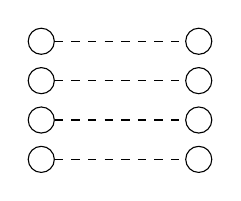
\begin{tikzpicture}[scale=1, auto=center]
\tikzstyle{every node}=[draw,shape=circle];
  \node[minimum size=0.25cm] (n1) at (0,1.5) {};
  \node[minimum size=0.25cm] (n2) at (0,1) {};
  \node[minimum size=0.25cm] (n3) at (0,0.5) {};
  \node[minimum size=0.25cm] (n4) at (0,0) {};
  \node[minimum size=0.25cm] (n5) at (2,1.5) {};
  \node[minimum size=0.25cm] (n6) at (2,1) {};
  \node[minimum size=0.25cm] (n7) at (2,0.5) {};
  \node[minimum size=0.25cm] (n8) at (2,0) {};

  \foreach \from/\to in {n1/n5,n2/n6,n3/n7,n4/n8}
    \draw[dashed] (\from) -- (\to);
  \foreach \from/\to in {}
    \draw (\from) -- (\to);
\end{tikzpicture}
\end{subfigure}
\begin{subfigure}{0.24\textwidth}
\centering
\caption{$G_2$: $1 / 6$}
\label{Fig1_2}

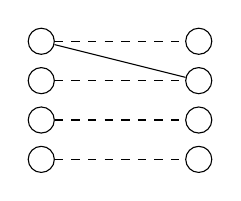
\begin{tikzpicture}[scale=1, auto=center]
\tikzstyle{every node}=[draw,shape=circle];
  \node[minimum size=0.25cm] (n1) at (0,1.5) {};
  \node[minimum size=0.25cm] (n2) at (0,1) {};
  \node[minimum size=0.25cm] (n3) at (0,0.5) {};
  \node[minimum size=0.25cm] (n4) at (0,0) {};
  \node[minimum size=0.25cm] (n5) at (2,1.5) {};
  \node[minimum size=0.25cm] (n6) at (2,1) {};
  \node[minimum size=0.25cm] (n7) at (2,0.5) {};
  \node[minimum size=0.25cm] (n8) at (2,0) {};

  \foreach \from/\to in {n1/n5,n2/n6,n3/n7,n4/n8}
    \draw[dashed] (\from) -- (\to);
  \foreach \from/\to in {n1/n6}
    \draw (\from) -- (\to);
\end{tikzpicture}
\end{subfigure}
\begin{subfigure}{0.24\textwidth}
\centering
\caption{$G_3$: $2 / 4$}
\label{Fig1_3}

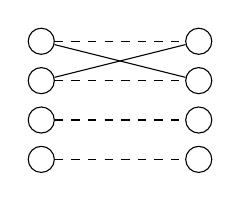
\begin{tikzpicture}[scale=1, auto=center]
\tikzstyle{every node}=[draw,shape=circle];
  \node[minimum size=0.25cm] (n1) at (0,1.5) {};
  \node[minimum size=0.25cm] (n2) at (0,1) {};
  \node[minimum size=0.25cm] (n3) at (0,0.5) {};
  \node[minimum size=0.25cm] (n4) at (0,0) {};
  \node[minimum size=0.25cm] (n5) at (2,1.5) {};
  \node[minimum size=0.25cm] (n6) at (2,1) {};
  \node[minimum size=0.25cm] (n7) at (2,0.5) {};
  \node[minimum size=0.25cm] (n8) at (2,0) {};

  \foreach \from/\to in {n1/n5,n2/n6,n3/n7,n4/n8}
    \draw[dashed] (\from) -- (\to);
  \foreach \from/\to in {n1/n6,n2/n5}
    \draw (\from) -- (\to);
\end{tikzpicture}
\end{subfigure}
\begin{subfigure}{0.24\textwidth}
\centering
\caption{$G_4$: $2 / 4$}
\label{Fig1_4}

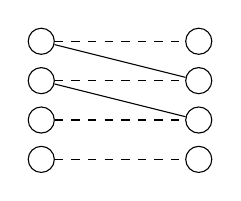
\begin{tikzpicture}[scale=1, auto=center]
\tikzstyle{every node}=[draw,shape=circle];
  \node[minimum size=0.25cm] (n1) at (0,1.5) {};
  \node[minimum size=0.25cm] (n2) at (0,1) {};
  \node[minimum size=0.25cm] (n3) at (0,0.5) {};
  \node[minimum size=0.25cm] (n4) at (0,0) {};
  \node[minimum size=0.25cm] (n5) at (2,1.5) {};
  \node[minimum size=0.25cm] (n6) at (2,1) {};
  \node[minimum size=0.25cm] (n7) at (2,0.5) {};
  \node[minimum size=0.25cm] (n8) at (2,0) {};

  \foreach \from/\to in {n1/n5,n2/n6,n3/n7,n4/n8}
    \draw[dashed] (\from) -- (\to);
  \foreach \from/\to in {n1/n6,n2/n7}
    \draw (\from) -- (\to);
\end{tikzpicture}
\end{subfigure}

%\vspace{0.25cm}
\begin{subfigure}{0.24\textwidth}
\centering
\caption{$G_5$: $2 / 5$}
\label{Fig1_5}

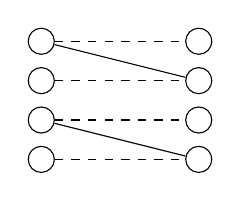
\begin{tikzpicture}[scale=1, auto=center]
\tikzstyle{every node}=[draw,shape=circle];
  \node[minimum size=0.25cm] (n1) at (0,1.5) {};
  \node[minimum size=0.25cm] (n2) at (0,1) {};
  \node[minimum size=0.25cm] (n3) at (0,0.5) {};
  \node[minimum size=0.25cm] (n4) at (0,0) {};
  \node[minimum size=0.25cm] (n5) at (2,1.5) {};
  \node[minimum size=0.25cm] (n6) at (2,1) {};
  \node[minimum size=0.25cm] (n7) at (2,0.5) {};
  \node[minimum size=0.25cm] (n8) at (2,0) {};

  \foreach \from/\to in {n1/n5,n2/n6,n3/n7,n4/n8}
    \draw[dashed] (\from) -- (\to);
  \foreach \from/\to in {n1/n6,n3/n8}
    \draw (\from) -- (\to);
\end{tikzpicture}
\end{subfigure}
\begin{subfigure}{0.24\textwidth}
\centering
\caption{$G_6$: $3 / 4$}
\label{Fig1_6}

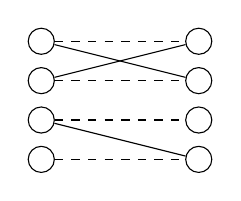
\begin{tikzpicture}[scale=1, auto=center]
\tikzstyle{every node}=[draw,shape=circle];
  \node[minimum size=0.25cm] (n1) at (0,1.5) {};
  \node[minimum size=0.25cm] (n2) at (0,1) {};
  \node[minimum size=0.25cm] (n3) at (0,0.5) {};
  \node[minimum size=0.25cm] (n4) at (0,0) {};
  \node[minimum size=0.25cm] (n5) at (2,1.5) {};
  \node[minimum size=0.25cm] (n6) at (2,1) {};
  \node[minimum size=0.25cm] (n7) at (2,0.5) {};
  \node[minimum size=0.25cm] (n8) at (2,0) {};

  \foreach \from/\to in {n1/n5,n2/n6,n3/n7,n4/n8}
    \draw[dashed] (\from) -- (\to);
  \foreach \from/\to in {n1/n6,n2/n5,n3/n8}
    \draw (\from) -- (\to);
\end{tikzpicture}
\end{subfigure}
\begin{subfigure}{0.24\textwidth}
\centering
\caption{$G_7$: $3 / 3$}
\label{Fig1_7}

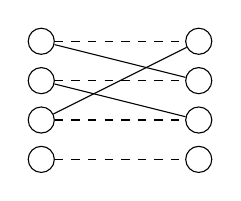
\begin{tikzpicture}[scale=1, auto=center]
\tikzstyle{every node}=[draw,shape=circle];
  \node[minimum size=0.25cm] (n1) at (0,1.5) {};
  \node[minimum size=0.25cm] (n2) at (0,1) {};
  \node[minimum size=0.25cm] (n3) at (0,0.5) {};
  \node[minimum size=0.25cm] (n4) at (0,0) {};
  \node[minimum size=0.25cm] (n5) at (2,1.5) {};
  \node[minimum size=0.25cm] (n6) at (2,1) {};
  \node[minimum size=0.25cm] (n7) at (2,0.5) {};
  \node[minimum size=0.25cm] (n8) at (2,0) {};

  \foreach \from/\to in {n1/n5,n2/n6,n3/n7,n4/n8}
    \draw[dashed] (\from) -- (\to);
  \foreach \from/\to in {n1/n6,n2/n7,n3/n5}
    \draw (\from) -- (\to);
\end{tikzpicture}
\end{subfigure}
\begin{subfigure}{0.24\textwidth}
\centering
\caption{$G_8$: $3 / 3$}
\label{Fig1_8}

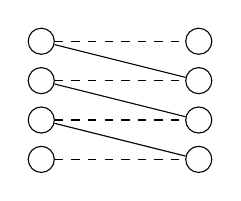
\begin{tikzpicture}[scale=1, auto=center]
\tikzstyle{every node}=[draw,shape=circle];
  \node[minimum size=0.25cm] (n1) at (0,1.5) {};
  \node[minimum size=0.25cm] (n2) at (0,1) {};
  \node[minimum size=0.25cm] (n3) at (0,0.5) {};
  \node[minimum size=0.25cm] (n4) at (0,0) {};
  \node[minimum size=0.25cm] (n5) at (2,1.5) {};
  \node[minimum size=0.25cm] (n6) at (2,1) {};
  \node[minimum size=0.25cm] (n7) at (2,0.5) {};
  \node[minimum size=0.25cm] (n8) at (2,0) {};

  \foreach \from/\to in {n1/n5,n2/n6,n3/n7,n4/n8}
    \draw[dashed] (\from) -- (\to);
  \foreach \from/\to in {n1/n6,n2/n7,n3/n8}
    \draw (\from) -- (\to);
\end{tikzpicture}
\end{subfigure}

%\vspace{0.25cm}
\begin{subfigure}{0.24\textwidth}
\centering
\caption{$G_9$: $4 / 2$}
\label{Fig1_9}

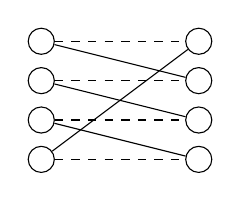
\begin{tikzpicture}[scale=1, auto=center]
\tikzstyle{every node}=[draw,shape=circle];
  \node[minimum size=0.25cm] (n1) at (0,1.5) {};
  \node[minimum size=0.25cm] (n2) at (0,1) {};
  \node[minimum size=0.25cm] (n3) at (0,0.5) {};
  \node[minimum size=0.25cm] (n4) at (0,0) {};
  \node[minimum size=0.25cm] (n5) at (2,1.5) {};
  \node[minimum size=0.25cm] (n6) at (2,1) {};
  \node[minimum size=0.25cm] (n7) at (2,0.5) {};
  \node[minimum size=0.25cm] (n8) at (2,0) {};

  \foreach \from/\to in {n1/n5,n2/n6,n3/n7,n4/n8}
    \draw[dashed] (\from) -- (\to);
  \foreach \from/\to in {n1/n6,n2/n7,n3/n8,n4/n5}
    \draw (\from) -- (\to);
\end{tikzpicture}
\end{subfigure}
\begin{subfigure}{0.24\textwidth}
\centering
\caption{$G_{10}$: $4 / 4$}
\label{Fig1_10}

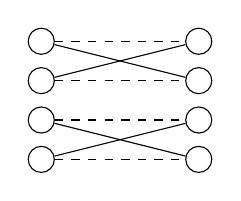
\begin{tikzpicture}[scale=1, auto=center]
\tikzstyle{every node}=[draw,shape=circle];
  \node[minimum size=0.25cm] (n1) at (0,1.5) {};
  \node[minimum size=0.25cm] (n2) at (0,1) {};
  \node[minimum size=0.25cm] (n3) at (0,0.5) {};
  \node[minimum size=0.25cm] (n4) at (0,0) {};
  \node[minimum size=0.25cm] (n5) at (2,1.5) {};
  \node[minimum size=0.25cm] (n6) at (2,1) {};
  \node[minimum size=0.25cm] (n7) at (2,0.5) {};
  \node[minimum size=0.25cm] (n8) at (2,0) {};

  \foreach \from/\to in {n1/n5,n2/n6,n3/n7,n4/n8}
    \draw[dashed] (\from) -- (\to);
  \foreach \from/\to in {n1/n6,n2/n5,n3/n8,n4/n7}
    \draw (\from) -- (\to);
\end{tikzpicture}
\end{subfigure}
\begin{subfigure}{0.24\textwidth}
\centering
\caption{$G_{11}$: $2 / 3$}
\label{Fig1_11}

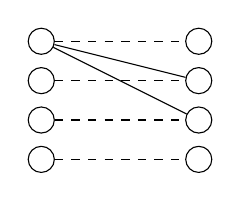
\begin{tikzpicture}[scale=1, auto=center]
\tikzstyle{every node}=[draw,shape=circle];
  \node[minimum size=0.25cm] (n1) at (0,1.5) {};
  \node[minimum size=0.25cm] (n2) at (0,1) {};
  \node[minimum size=0.25cm] (n3) at (0,0.5) {};
  \node[minimum size=0.25cm] (n4) at (0,0) {};
  \node[minimum size=0.25cm] (n5) at (2,1.5) {};
  \node[minimum size=0.25cm] (n6) at (2,1) {};
  \node[minimum size=0.25cm] (n7) at (2,0.5) {};
  \node[minimum size=0.25cm] (n8) at (2,0) {};

  \foreach \from/\to in {n1/n5,n2/n6,n3/n7,n4/n8}
    \draw[dashed] (\from) -- (\to);  
  \foreach \from/\to in {n1/n6,n1/n7}
    \draw (\from) -- (\to);
\end{tikzpicture}
\end{subfigure}
\begin{subfigure}{0.24\textwidth}
\centering
\caption{$G_{12}$: $3 / 2$}
\label{Fig1_12}

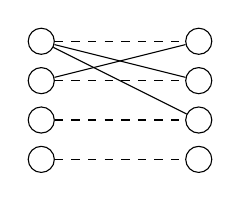
\begin{tikzpicture}[scale=1, auto=center]
\tikzstyle{every node}=[draw,shape=circle];
  \node[minimum size=0.25cm] (n1) at (0,1.5) {};
  \node[minimum size=0.25cm] (n2) at (0,1) {};
  \node[minimum size=0.25cm] (n3) at (0,0.5) {};
  \node[minimum size=0.25cm] (n4) at (0,0) {};
  \node[minimum size=0.25cm] (n5) at (2,1.5) {};
  \node[minimum size=0.25cm] (n6) at (2,1) {};
  \node[minimum size=0.25cm] (n7) at (2,0.5) {};
  \node[minimum size=0.25cm] (n8) at (2,0) {};

  \foreach \from/\to in {n1/n5,n2/n6,n3/n7,n4/n8}
    \draw[dashed] (\from) -- (\to);
  \foreach \from/\to in {n1/n6,n1/n7,n2/n5}
    \draw (\from) -- (\to);
\end{tikzpicture}
\end{subfigure}

%\vspace{0.25cm}
\begin{subfigure}{0.24\textwidth}
\centering
\caption{$G_{13}$: $3 / 3$}
\label{Fig1_13}

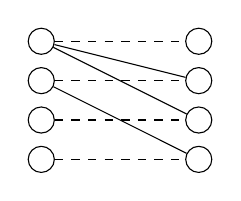
\begin{tikzpicture}[scale=1, auto=center]
\tikzstyle{every node}=[draw,shape=circle];
  \node[minimum size=0.25cm] (n1) at (0,1.5) {};
  \node[minimum size=0.25cm] (n2) at (0,1) {};
  \node[minimum size=0.25cm] (n3) at (0,0.5) {};
  \node[minimum size=0.25cm] (n4) at (0,0) {};
  \node[minimum size=0.25cm] (n5) at (2,1.5) {};
  \node[minimum size=0.25cm] (n6) at (2,1) {};
  \node[minimum size=0.25cm] (n7) at (2,0.5) {};
  \node[minimum size=0.25cm] (n8) at (2,0) {};

  \foreach \from/\to in {n1/n5,n2/n6,n3/n7,n4/n8}
    \draw[dashed] (\from) -- (\to);
  \foreach \from/\to in {n1/n6,n1/n7,n2/n8}
    \draw (\from) -- (\to);
\end{tikzpicture}
\end{subfigure}
\begin{subfigure}{0.24\textwidth}
\centering
\caption{$G_{14}$: $3 / 2$}
\label{Fig1_14}

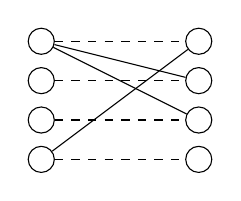
\begin{tikzpicture}[scale=1, auto=center]
\tikzstyle{every node}=[draw,shape=circle];
  \node[minimum size=0.25cm] (n1) at (0,1.5) {};
  \node[minimum size=0.25cm] (n2) at (0,1) {};
  \node[minimum size=0.25cm] (n3) at (0,0.5) {};
  \node[minimum size=0.25cm] (n4) at (0,0) {};
  \node[minimum size=0.25cm] (n5) at (2,1.5) {};
  \node[minimum size=0.25cm] (n6) at (2,1) {};
  \node[minimum size=0.25cm] (n7) at (2,0.5) {};
  \node[minimum size=0.25cm] (n8) at (2,0) {};

  \foreach \from/\to in {n1/n5,n2/n6,n3/n7,n4/n8}
    \draw[dashed] (\from) -- (\to);
  \foreach \from/\to in {n1/n6,n1/n7,n4/n5}
    \draw (\from) -- (\to);
\end{tikzpicture}
\end{subfigure}
\begin{subfigure}{0.24\textwidth}
\centering
\caption{$G_{15}$: $4 / 2$}
\label{Fig1_15}

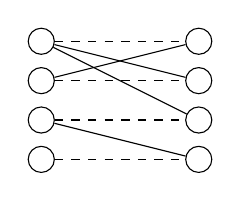
\begin{tikzpicture}[scale=1, auto=center]
\tikzstyle{every node}=[draw,shape=circle];
  \node[minimum size=0.25cm] (n1) at (0,1.5) {};
  \node[minimum size=0.25cm] (n2) at (0,1) {};
  \node[minimum size=0.25cm] (n3) at (0,0.5) {};
  \node[minimum size=0.25cm] (n4) at (0,0) {};
  \node[minimum size=0.25cm] (n5) at (2,1.5) {};
  \node[minimum size=0.25cm] (n6) at (2,1) {};
  \node[minimum size=0.25cm] (n7) at (2,0.5) {};
  \node[minimum size=0.25cm] (n8) at (2,0) {};

  \foreach \from/\to in {n1/n5,n2/n6,n3/n7,n4/n8}
    \draw[dashed] (\from) -- (\to); 
  \foreach \from/\to in {n1/n6,n1/n7,n2/n5,n3/n8}
    \draw (\from) -- (\to);
\end{tikzpicture}
\end{subfigure}
\begin{subfigure}{0.24\textwidth}
\centering
\caption{$G_{16}$: $4 / 2$}
\label{Fig1_16}

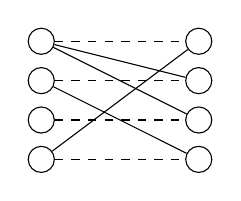
\begin{tikzpicture}[scale=1, auto=center]
\tikzstyle{every node}=[draw,shape=circle];
  \node[minimum size=0.25cm] (n1) at (0,1.5) {};
  \node[minimum size=0.25cm] (n2) at (0,1) {};
  \node[minimum size=0.25cm] (n3) at (0,0.5) {};
  \node[minimum size=0.25cm] (n4) at (0,0) {};
  \node[minimum size=0.25cm] (n5) at (2,1.5) {};
  \node[minimum size=0.25cm] (n6) at (2,1) {};
  \node[minimum size=0.25cm] (n7) at (2,0.5) {};
  \node[minimum size=0.25cm] (n8) at (2,0) {};

  \foreach \from/\to in {n1/n5,n2/n6,n3/n7,n4/n8}
    \draw[dashed] (\from) -- (\to);
  \foreach \from/\to in {n1/n6,n1/n7,n2/n8,n4/n5}
    \draw (\from) -- (\to);
\end{tikzpicture}
\end{subfigure}

%\vspace{0.25cm}
\begin{subfigure}{0.24\textwidth}
\centering
\caption{$G_{17}$: $4 / 2$}
\label{Fig1_17}

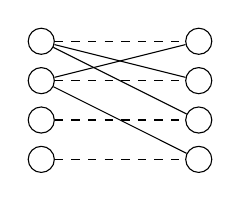
\begin{tikzpicture}[scale=1, auto=center]
\tikzstyle{every node}=[draw,shape=circle];
  \node[minimum size=0.25cm] (n1) at (0,1.5) {};
  \node[minimum size=0.25cm] (n2) at (0,1) {};
  \node[minimum size=0.25cm] (n3) at (0,0.5) {};
  \node[minimum size=0.25cm] (n4) at (0,0) {};
  \node[minimum size=0.25cm] (n5) at (2,1.5) {};
  \node[minimum size=0.25cm] (n6) at (2,1) {};
  \node[minimum size=0.25cm] (n7) at (2,0.5) {};
  \node[minimum size=0.25cm] (n8) at (2,0) {};

  \foreach \from/\to in {n1/n5,n2/n6,n3/n7,n4/n8}
    \draw[dashed] (\from) -- (\to);
  \foreach \from/\to in {n1/n6,n1/n7,n2/n5,n2/n8}
    \draw (\from) -- (\to);
\end{tikzpicture}
\end{subfigure}
\begin{subfigure}{0.24\textwidth}
\centering
\caption{$G_{18}$: $4 / 1$}
\label{Fig1_18}

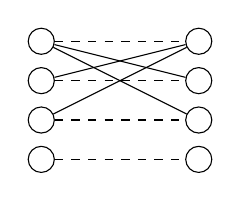
\begin{tikzpicture}[scale=1, auto=center]
\tikzstyle{every node}=[draw,shape=circle];
  \node[minimum size=0.25cm] (n1) at (0,1.5) {};
  \node[minimum size=0.25cm] (n2) at (0,1) {};
  \node[minimum size=0.25cm] (n3) at (0,0.5) {};
  \node[minimum size=0.25cm] (n4) at (0,0) {};
  \node[minimum size=0.25cm] (n5) at (2,1.5) {};
  \node[minimum size=0.25cm] (n6) at (2,1) {};
  \node[minimum size=0.25cm] (n7) at (2,0.5) {};
  \node[minimum size=0.25cm] (n8) at (2,0) {};

  \foreach \from/\to in {n1/n5,n2/n6,n3/n7,n4/n8}
    \draw[dashed] (\from) -- (\to);
  \foreach \from/\to in {n1/n6,n1/n7,n2/n5,n3/n5}
    \draw (\from) -- (\to);
\end{tikzpicture}
\end{subfigure}
\begin{subfigure}{0.24\textwidth}
\centering
\caption{$G_{19}$: $4 / 1$}
\label{Fig1_19}

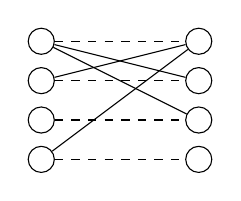
\begin{tikzpicture}[scale=1, auto=center]
\tikzstyle{every node}=[draw,shape=circle];
  \node[minimum size=0.25cm] (n1) at (0,1.5) {};
  \node[minimum size=0.25cm] (n2) at (0,1) {};
  \node[minimum size=0.25cm] (n3) at (0,0.5) {};
  \node[minimum size=0.25cm] (n4) at (0,0) {};
  \node[minimum size=0.25cm] (n5) at (2,1.5) {};
  \node[minimum size=0.25cm] (n6) at (2,1) {};
  \node[minimum size=0.25cm] (n7) at (2,0.5) {};
  \node[minimum size=0.25cm] (n8) at (2,0) {};

  \foreach \from/\to in {n1/n5,n2/n6,n3/n7,n4/n8}
    \draw[dashed] (\from) -- (\to); 
  \foreach \from/\to in {n1/n6,n1/n7,n2/n5,n4/n5}
    \draw (\from) -- (\to);
\end{tikzpicture}
\end{subfigure}
\begin{subfigure}{0.24\textwidth}
\centering
\caption{$G_{20}$: $4 / 3$}
\label{Fig1_20}

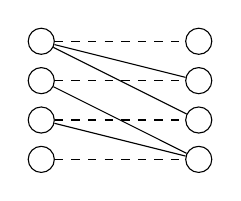
\begin{tikzpicture}[scale=1, auto=center]
\tikzstyle{every node}=[draw,shape=circle];
  \node[minimum size=0.25cm] (n1) at (0,1.5) {};
  \node[minimum size=0.25cm] (n2) at (0,1) {};
  \node[minimum size=0.25cm] (n3) at (0,0.5) {};
  \node[minimum size=0.25cm] (n4) at (0,0) {};
  \node[minimum size=0.25cm] (n5) at (2,1.5) {};
  \node[minimum size=0.25cm] (n6) at (2,1) {};
  \node[minimum size=0.25cm] (n7) at (2,0.5) {};
  \node[minimum size=0.25cm] (n8) at (2,0) {};

  \foreach \from/\to in {n1/n5,n2/n6,n3/n7,n4/n8}
    \draw[dashed] (\from) -- (\to);
  \foreach \from/\to in {n1/n6,n1/n7,n2/n8,n3/n8}
    \draw (\from) -- (\to);
\end{tikzpicture}
\end{subfigure}

%\vspace{0.25cm}
\begin{subfigure}{0.24\textwidth}
\centering
\caption{$G_{21}$: $5 / 1$}
\label{Fig1_21}

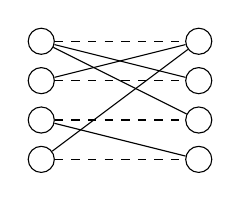
\begin{tikzpicture}[scale=1, auto=center]
\tikzstyle{every node}=[draw,shape=circle];
  \node[minimum size=0.25cm] (n1) at (0,1.5) {};
  \node[minimum size=0.25cm] (n2) at (0,1) {};
  \node[minimum size=0.25cm] (n3) at (0,0.5) {};
  \node[minimum size=0.25cm] (n4) at (0,0) {};
  \node[minimum size=0.25cm] (n5) at (2,1.5) {};
  \node[minimum size=0.25cm] (n6) at (2,1) {};
  \node[minimum size=0.25cm] (n7) at (2,0.5) {};
  \node[minimum size=0.25cm] (n8) at (2,0) {};

  \foreach \from/\to in {n1/n5,n2/n6,n3/n7,n4/n8}
    \draw[dashed] (\from) -- (\to);
  \foreach \from/\to in {n1/n6,n1/n7,n2/n5,n4/n5,n3/n8}
    \draw (\from) -- (\to);
\end{tikzpicture}
\end{subfigure}
\begin{subfigure}{0.24\textwidth}
\centering
\caption{$G_{22}$: $5 / 2$}
\label{Fig1_22}

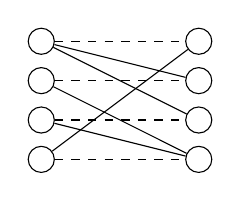
\begin{tikzpicture}[scale=1, auto=center]
\tikzstyle{every node}=[draw,shape=circle];
  \node[minimum size=0.25cm] (n1) at (0,1.5) {};
  \node[minimum size=0.25cm] (n2) at (0,1) {};
  \node[minimum size=0.25cm] (n3) at (0,0.5) {};
  \node[minimum size=0.25cm] (n4) at (0,0) {};
  \node[minimum size=0.25cm] (n5) at (2,1.5) {};
  \node[minimum size=0.25cm] (n6) at (2,1) {};
  \node[minimum size=0.25cm] (n7) at (2,0.5) {};
  \node[minimum size=0.25cm] (n8) at (2,0) {};

  \foreach \from/\to in {n1/n5,n2/n6,n3/n7,n4/n8}
    \draw[dashed] (\from) -- (\to);
  \foreach \from/\to in {n1/n6,n1/n7,n2/n8,n3/n8,n4/n5}
    \draw (\from) -- (\to);
\end{tikzpicture}
\end{subfigure}
\begin{subfigure}{0.24\textwidth}
\centering
\caption{$G_{23}$: $4 / 1$}
\label{Fig1_23}

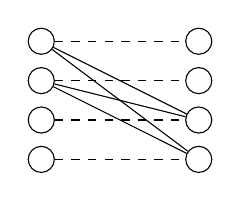
\begin{tikzpicture}[scale=1, auto=center]
\tikzstyle{every node}=[draw,shape=circle];
  \node[minimum size=0.25cm] (n1) at (0,1.5) {};
  \node[minimum size=0.25cm] (n2) at (0,1) {};
  \node[minimum size=0.25cm] (n3) at (0,0.5) {};
  \node[minimum size=0.25cm] (n4) at (0,0) {};
  \node[minimum size=0.25cm] (n5) at (2,1.5) {};
  \node[minimum size=0.25cm] (n6) at (2,1) {};
  \node[minimum size=0.25cm] (n7) at (2,0.5) {};
  \node[minimum size=0.25cm] (n8) at (2,0) {};

  \foreach \from/\to in {n1/n5,n2/n6,n3/n7,n4/n8}
    \draw[dashed] (\from) -- (\to); 
  \foreach \from/\to in {n1/n7,n1/n8,n2/n7,n2/n8} 
    \draw (\from) -- (\to);
\end{tikzpicture}
\end{subfigure}
\begin{subfigure}{0.24\textwidth}
\centering
\caption{$G_{24}$: $5 / 1$}
\label{Fig1_24}

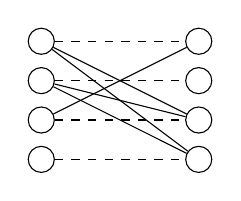
\begin{tikzpicture}[scale=1, auto=center]
\tikzstyle{every node}=[draw,shape=circle];
  \node[minimum size=0.25cm] (n1) at (0,1.5) {};
  \node[minimum size=0.25cm] (n2) at (0,1) {};
  \node[minimum size=0.25cm] (n3) at (0,0.5) {};
  \node[minimum size=0.25cm] (n4) at (0,0) {};
  \node[minimum size=0.25cm] (n5) at (2,1.5) {};
  \node[minimum size=0.25cm] (n6) at (2,1) {};
  \node[minimum size=0.25cm] (n7) at (2,0.5) {};
  \node[minimum size=0.25cm] (n8) at (2,0) {};

  \foreach \from/\to in {n1/n5,n2/n6,n3/n7,n4/n8}
    \draw[dashed] (\from) -- (\to);
  \foreach \from/\to in {n1/n7,n1/n8,n2/n7,n2/n8,n3/n5}
    \draw (\from) -- (\to);
\end{tikzpicture}
\end{subfigure}

%\vspace{0.25cm}
\begin{subfigure}{0.24\textwidth}
\centering
\caption{$G_{25}$: $6 / 1$}
\label{Fig1_25}

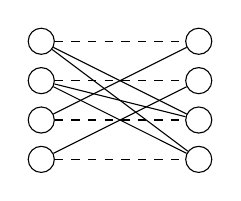
\begin{tikzpicture}[scale=1, auto=center]
\tikzstyle{every node}=[draw,shape=circle];
  \node[minimum size=0.25cm] (n1) at (0,1.5) {};
  \node[minimum size=0.25cm] (n2) at (0,1) {};
  \node[minimum size=0.25cm] (n3) at (0,0.5) {};
  \node[minimum size=0.25cm] (n4) at (0,0) {};
  \node[minimum size=0.25cm] (n5) at (2,1.5) {};
  \node[minimum size=0.25cm] (n6) at (2,1) {};
  \node[minimum size=0.25cm] (n7) at (2,0.5) {};
  \node[minimum size=0.25cm] (n8) at (2,0) {};

  \foreach \from/\to in {n1/n5,n2/n6,n3/n7,n4/n8}
    \draw[dashed] (\from) -- (\to);
  \foreach \from/\to in {n1/n7,n1/n8,n2/n7,n2/n8,n3/n5,n4/n6}
    \draw (\from) -- (\to);
\end{tikzpicture}
\end{subfigure}
\begin{subfigure}{0.24\textwidth}
\centering
\caption{$G_{26}$: $6 / 1$}
\label{Fig1_26}

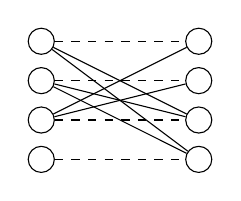
\begin{tikzpicture}[scale=1, auto=center]
\tikzstyle{every node}=[draw,shape=circle];
  \node[minimum size=0.25cm] (n1) at (0,1.5) {};
  \node[minimum size=0.25cm] (n2) at (0,1) {};
  \node[minimum size=0.25cm] (n3) at (0,0.5) {};
  \node[minimum size=0.25cm] (n4) at (0,0) {};
  \node[minimum size=0.25cm] (n5) at (2,1.5) {};
  \node[minimum size=0.25cm] (n6) at (2,1) {};
  \node[minimum size=0.25cm] (n7) at (2,0.5) {};
  \node[minimum size=0.25cm] (n8) at (2,0) {};

  \foreach \from/\to in {n1/n5,n2/n6,n3/n7,n4/n8}
    \draw[dashed] (\from) -- (\to);
  \foreach \from/\to in {n1/n7,n1/n8,n2/n7,n2/n8,n3/n5,n3/n6}
    \draw (\from) -- (\to);
\end{tikzpicture}
\end{subfigure}
\begin{subfigure}{0.24\textwidth}
\centering
\caption{$G_{27}$: $8 / 1$}
\label{Fig1_27}

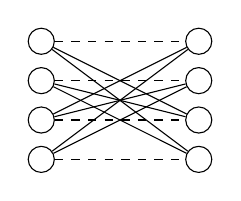
\begin{tikzpicture}[scale=1, auto=center]
\tikzstyle{every node}=[draw,shape=circle];
  \node[minimum size=0.25cm] (n1) at (0,1.5) {};
  \node[minimum size=0.25cm] (n2) at (0,1) {};
  \node[minimum size=0.25cm] (n3) at (0,0.5) {};
  \node[minimum size=0.25cm] (n4) at (0,0) {};
  \node[minimum size=0.25cm] (n5) at (2,1.5) {};
  \node[minimum size=0.25cm] (n6) at (2,1) {};
  \node[minimum size=0.25cm] (n7) at (2,0.5) {};
  \node[minimum size=0.25cm] (n8) at (2,0) {};

  \foreach \from/\to in {n1/n5,n2/n6,n3/n7,n4/n8}
    \draw[dashed] (\from) -- (\to); 
  \foreach \from/\to in {n1/n7,n1/n8,n2/n7,n2/n8,n3/n5,n3/n6,n4/n5,n4/n6} 
    \draw (\from) -- (\to);
\end{tikzpicture}
\end{subfigure}
\begin{subfigure}{0.24\textwidth}
\centering
\caption{$G_{28}$: $3 / 0$}
\label{Fig1_28}

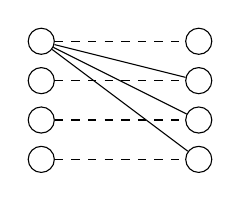
\begin{tikzpicture}[scale=1, auto=center]
\tikzstyle{every node}=[draw,shape=circle];
  \node[minimum size=0.25cm] (n1) at (0,1.5) {};
  \node[minimum size=0.25cm] (n2) at (0,1) {};
  \node[minimum size=0.25cm] (n3) at (0,0.5) {};
  \node[minimum size=0.25cm] (n4) at (0,0) {};
  \node[minimum size=0.25cm] (n5) at (2,1.5) {};
  \node[minimum size=0.25cm] (n6) at (2,1) {};
  \node[minimum size=0.25cm] (n7) at (2,0.5) {};
  \node[minimum size=0.25cm] (n8) at (2,0) {};

  \foreach \from/\to in {n1/n5,n2/n6,n3/n7,n4/n8}
    \draw[dashed] (\from) -- (\to);
  \foreach \from/\to in {n1/n6,n1/n7,n1/n8}
    \draw (\from) -- (\to);
\end{tikzpicture}
\end{subfigure}

%\vspace{0.25cm}
\begin{subfigure}{0.24\textwidth}
\centering
\caption{$G_{29}$: $4 / 0$}
\label{Fig1_29}

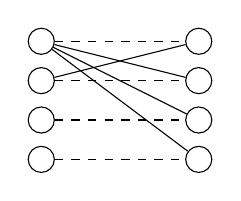
\begin{tikzpicture}[scale=1, auto=center]
\tikzstyle{every node}=[draw,shape=circle];
  \node[minimum size=0.25cm] (n1) at (0,1.5) {};
  \node[minimum size=0.25cm] (n2) at (0,1) {};
  \node[minimum size=0.25cm] (n3) at (0,0.5) {};
  \node[minimum size=0.25cm] (n4) at (0,0) {};
  \node[minimum size=0.25cm] (n5) at (2,1.5) {};
  \node[minimum size=0.25cm] (n6) at (2,1) {};
  \node[minimum size=0.25cm] (n7) at (2,0.5) {};
  \node[minimum size=0.25cm] (n8) at (2,0) {};

  \foreach \from/\to in {n1/n5,n2/n6,n3/n7,n4/n8}
    \draw[dashed] (\from) -- (\to);
  \foreach \from/\to in {n1/n6,n1/n7,n1/n8,n2/n5}
    \draw (\from) -- (\to);
\end{tikzpicture}
\end{subfigure}
\begin{subfigure}{0.24\textwidth}
\centering
\caption{$G_{30}$: $5 / 0$}
\label{Fig1_30}

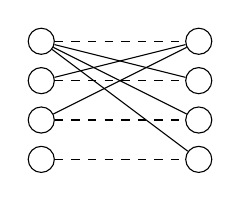
\begin{tikzpicture}[scale=1, auto=center]
\tikzstyle{every node}=[draw,shape=circle];
  \node[minimum size=0.25cm] (n1) at (0,1.5) {};
  \node[minimum size=0.25cm] (n2) at (0,1) {};
  \node[minimum size=0.25cm] (n3) at (0,0.5) {};
  \node[minimum size=0.25cm] (n4) at (0,0) {};
  \node[minimum size=0.25cm] (n5) at (2,1.5) {};
  \node[minimum size=0.25cm] (n6) at (2,1) {};
  \node[minimum size=0.25cm] (n7) at (2,0.5) {};
  \node[minimum size=0.25cm] (n8) at (2,0) {};

  \foreach \from/\to in {n1/n5,n2/n6,n3/n7,n4/n8}
    \draw[dashed] (\from) -- (\to);
  \foreach \from/\to in {n1/n6,n1/n7,n1/n8,n2/n5,n3/n5}
    \draw (\from) -- (\to);
\end{tikzpicture}
\end{subfigure}
\begin{subfigure}{0.24\textwidth}
\centering
\caption{$G_{31}$: $6 / 0$}
\label{Fig1_31}

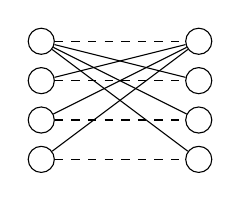
\begin{tikzpicture}[scale=1, auto=center]
\tikzstyle{every node}=[draw,shape=circle];
  \node[minimum size=0.25cm] (n1) at (0,1.5) {};
  \node[minimum size=0.25cm] (n2) at (0,1) {};
  \node[minimum size=0.25cm] (n3) at (0,0.5) {};
  \node[minimum size=0.25cm] (n4) at (0,0) {};
  \node[minimum size=0.25cm] (n5) at (2,1.5) {};
  \node[minimum size=0.25cm] (n6) at (2,1) {};
  \node[minimum size=0.25cm] (n7) at (2,0.5) {};
  \node[minimum size=0.25cm] (n8) at (2,0) {};

  \foreach \from/\to in {n1/n5,n2/n6,n3/n7,n4/n8}
    \draw[dashed] (\from) -- (\to); 
  \foreach \from/\to in {n1/n6,n1/n7,n1/n8,n2/n5,n3/n5,n4/n5} 
    \draw (\from) -- (\to);
\end{tikzpicture}
\end{subfigure}

\captionsetup{justification=centerfirst}
\caption{Balanced bipartite graphs with eight nodes, pair and type constraints \\ \vspace{0.2cm}
\footnotesize{\emph{Notes}: Dashed lines indicate the pair constraints, solid lines indicate the type constraints. \\
%Group winners are the nodes on the left-hand side, runners-up are the nodes on the right-hand side. \\
The first (second) number shows the number of type exclusions (the number of valid assignments).}}
\label{Fig1}
\end{figure}

%\end{document}